\documentclass[8pt,a4paper,compress]{beamer}

\usepackage{/home/siyer/lib/slides}

\title{Basic Data Structures}
\date{}

\begin{document}
\begin{frame}
\vfill
\titlepage
\end{frame}

\begin{frame}
\frametitle{Outline}
\tableofcontents
\end{frame}

\section{Some Java Preliminaries}
\begin{frame}[fragile]
\pause

Generics (aka parametrized types) is a Java mechanism that enables the implementation of collection ADTs that can store any type of data

\begin{lstlisting}[language=Java]
Stack<String> s1 = new Stack<String>();
Stack<Date> s2 = new Stack<Date>();
s1.push("Test");
s2.push(new Date(3, 14, 1879));
String s = s1.pop();
Date d = s2.pop();
\end{lstlisting}

\pause
\bigskip

Since generics are reference types, Java allows generic code to be used with primitive types by automatically converting (auto boxing) them to their corresponding (wrapper) reference types and vice versa (auto unboxing)
\begin{lstlisting}[language=Java]
Stack<Integer> stack = new Stack<Integer>();
stack.push(42);      // auto boxing (int -> Integer)
int i = stack.pop(); // auto unboxing (Integer -> int)
\end{lstlisting}

\pause
\bigskip

Iterable collections can be enumerated using foreach statement 
\begin{lstlisting}[language=Java]
Bag<Integer> numbers = new Bag<Integer>();
...
for (int x : numbers) { StdOut.println(x); }
\end{lstlisting}

which (roughly) translates to 

\begin{lstlisting}[language=Java]
Iterator<Integer> iter = numbers.iterator();
while (iter.hasNext()) { StdOut.println(iter.next()); }
\end{lstlisting}
\end{frame}

\section{Linked Lists}
\begin{frame}[fragile]
\pause

A linked list is a recursive data structure that is either empty (\lstinline{null}) or a reference to a node having a generic item and a reference to a linked list

\pause
\bigskip

Node record 
\begin{lstlisting}[language=Java]
private class Node {
    Item item; // generic item
    Node next;
}
\end{lstlisting}

\pause
\bigskip

Traversal
\begin{lstlisting}[language=Java]
for (Node x = first; x != null; x = x.next) {

    // do something with x.item.
    
}
\end{lstlisting}
\end{frame}

\begin{frame}[fragile]
\pause

Building a linked list
\begin{lstlisting}[language=Java]
Node first = new Node();
first.item = "to";
\end{lstlisting}

\begin{center}
\visible<2->{\includegraphics[scale=0.7]{{./figures/llist1.1}.pdf}}
\end{center}

\pause

\begin{lstlisting}[language=Java]
Node second = new Node();
second.item = "be";
first.next = second;
\end{lstlisting}

\begin{center}
\visible<3->{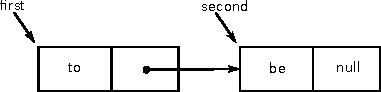
\includegraphics[scale=0.7]{{./figures/llist1.2}.pdf}}
\end{center}

\pause

\begin{lstlisting}[language=Java]
Node third = new Node();
third.item = "or";
second.next = third;
\end{lstlisting}

\begin{center}
\visible<4->{\includegraphics[scale=0.7]{{./figures/llist1.3}.pdf}}
\end{center}
\end{frame}

\begin{frame}[fragile]
\pause

Insert at the beginning
\begin{lstlisting}[language=Java]
Node oldfirst = first;
\end{lstlisting}

\begin{center}
\visible<2->{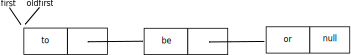
\includegraphics[scale=0.7]{{./figures/llist2.1}.pdf}}
\end{center}

\pause

\begin{lstlisting}[language=Java]
first = new Node();
first.item = "not";
\end{lstlisting}

\begin{center}
\visible<3->{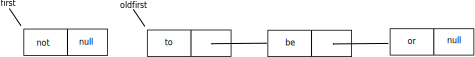
\includegraphics[scale=0.7]{{./figures/llist2.2}.pdf}}
\end{center}

\pause

\begin{lstlisting}[language=Java]
first.next = oldfirst;
\end{lstlisting}

\begin{center}
\visible<4->{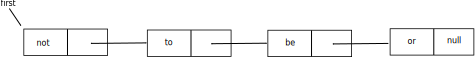
\includegraphics[scale=0.7]{{./figures/llist2.3}.pdf}}
\end{center}
\end{frame}

\begin{frame}[fragile]
\pause

Remove from the beginning
\begin{lstlisting}[language=Java]
first = first.next;
\end{lstlisting}

\begin{center}
\visible<2->{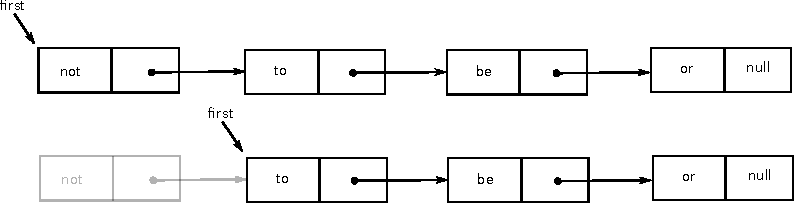
\includegraphics[scale=0.7]{./figures/llist3.pdf}}
\end{center}
\end{frame}

\begin{frame}[fragile]
\pause

Insert at the end
\begin{lstlisting}[language=Java]
Node oldlast = last;
\end{lstlisting}

\begin{center}
\visible<2->{\includegraphics[scale=0.7]{{./figures/llist4.1}.pdf}}
\end{center}

\pause

\begin{lstlisting}[language=Java]
last = new Node();
last.item = "not";
\end{lstlisting}

\begin{center}
\visible<3->{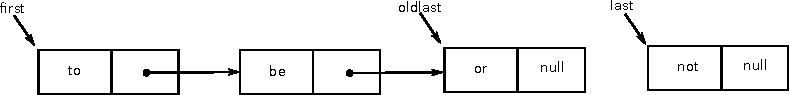
\includegraphics[scale=0.7]{{./figures/llist4.2}.pdf}}
\end{center}

\pause

\begin{lstlisting}[language=Java]
oldlast.next = last;
\end{lstlisting}

\begin{center}
\visible<4->{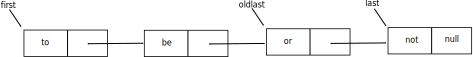
\includegraphics[scale=0.7]{{./figures/llist4.3}.pdf}}
\end{center}
\end{frame}

\section{Bags}
\begin{frame}[fragile]
\pause

A \lstinline{Bag} is an iterable collection that provides clients the ability to collect items
\begin{center}
\begin{tabular}{cc}
method & description \\ \hline
\lstinline$Bag<Item>()$ & construct an empty bag \\
\lstinline$boolean isEmpty()$ & is the bag empty? \\
\lstinline$int size()$ & number of items in the bag \\
\lstinline$void add(Item item)$ & add $item$ to the bag \\
\lstinline$Iterator<Item> iterator()$ & an iterator over the items in the bag
\end{tabular} 
\end{center}

\pause

\lstinline{Bag} client
\begin{lstlisting}[language=Java]
import edu.princeton.cs.algs4.LinkedBag;
import edu.princeton.cs.algs4.StdIn;
import edu.princeton.cs.algs4.StdOut;

public class Stats {
    public static void main(String[] args) {
        LinkedBag<Double> numbers = new LinkedBag<Double>();
        while (!StdIn.isEmpty()) { numbers.add(StdIn.readDouble()); }
        int N = numbers.size();
        double sum = 0.0;
        for (double x : numbers) { sum += x; }
        double mean = sum / N;
        sum = 0.0;
        for (double x : numbers) { sum += (x - mean) * (x - mean); }
        double std = Math.sqrt(sum / (N - 1));
        StdOut.printf("Mean:    %.2f\n", mean);
        StdOut.printf("Std dev: %.2f\n", std);
    }
}
\end{lstlisting}

\pause

\begin{lstlisting}[language={}]
$ java Stats
100 99 101 120 98 107 109 81 101 90 <ctrl-d>
Mean:    100.60
Std dev: 10.51
\end{lstlisting}
\end{frame}

\begin{frame}[fragile]
\pause

\lstinline{Bag} implementation using a linked list
\begin{lstlisting}[language=Java]
package edu.princeton.cs.algs4;

import java.util.Iterator;
import java.util.NoSuchElementException;

public class LinkedBag<Item> implements Iterable<Item> {
    private Node first;
    private int N;

    private class Node {
        private Item item;
        private Node next;
    }

    public LinkedBag() {
        first = null;
        N = 0;
    }

    public boolean isEmpty() { return first == null; }

    public int size() { return N; }

    public void add(Item item) {
        Node oldfirst = first;
        first = new Node();
        first.item = item;
        first.next = oldfirst;
        N++;
    }
\end{lstlisting}
\end{frame}

\begin{frame}[fragile]
\pause

\begin{lstlisting}[language=Java]
    public Iterator<Item> iterator() { return new ListIterator<Item>(first); }

    private class ListIterator<Item> implements Iterator<Item> {
        private Node current;

        public ListIterator(Node first) { current = first; }

        public boolean hasNext() { return current != null; }

        public Item next() {
            if (!hasNext()) { throw new NoSuchElementException(); }
            Item item = current.item;
            current = current.next; 
            return item;
        }
    }
}
\end{lstlisting}
\end{frame}

\begin{frame}[fragile]
\pause

\lstinline{Bag} implementation using a resizing array
\begin{lstlisting}[language=Java]
package edu.princeton.cs.algs4;

import java.util.Iterator;
import java.util.NoSuchElementException;

public class ResizingArrayBag<Item> implements Iterable<Item> {
    private Item[] a; 
    private int N;  

    public ResizingArrayBag() {
        a = (Item[]) new Object[2];
        N = 0;
    }

    public boolean isEmpty() { return N == 0; }

    public int size() { return N; }

    private void resize(int capacity) {
        Item[] temp = (Item[]) new Object[capacity];
        for (int i = 0; i < N; i++) { temp[i] = a[i]; }
        a = temp;
    }

    public void add(Item item) {
        if (N == a.length) { resize(2 * a.length); }
        a[N++] = item; 
    }
\end{lstlisting}
\end{frame}

\begin{frame}[fragile]
\pause

\begin{lstlisting}[language=Java]
    public Iterator<Item> iterator() { return new ArrayIterator(); }

    private class ArrayIterator implements Iterator<Item> {
        private int i = 0;

        public boolean hasNext()  { return i < N; }
        
        public Item next() {
            if (!hasNext()) { throw new NoSuchElementException(); }
            return a[i++];
        }
    }
}
\end{lstlisting}
\end{frame}

\section{Queues}
\begin{frame}[fragile]
\pause

A \lstinline{Queue} is an iterable collection that is based on the first-in-first-out (FIFO) policy
\begin{center}
\begin{tabular}{cc}
method & description \\ \hline
\lstinline$Queue<Item>()$ & construct an empty queue \\
\lstinline$boolean isEmpty()$ & is the queue empty? \\
\lstinline$int size()$ & number of items in the queue \\
\lstinline$void enqueue(Item item)$ & add $item$ to the queue \\
\lstinline$Item dequeue()$ & remove the least recently added item \\
\lstinline$Iterator<Item> iterator()$ & an iterator over the items in the queue
\end{tabular} 
\end{center}

\pause

\lstinline{Queue} client
\begin{lstlisting}[language=Java]
import edu.princeton.cs.algs4.LinkedQueue;
import edu.princeton.cs.algs4.StdIn;
import edu.princeton.cs.algs4.StdOut;

public class ReadInts {
    public static void main(String[] args) {
        LinkedQueue<Integer> q = new LinkedQueue<Integer>();
        while (!StdIn.isEmpty()) { q.enqueue(StdIn.readInt()); }
        for (int i : q) { StdOut.println(i); }
    }
}
\end{lstlisting}

\pause

\begin{lstlisting}[language={}]
$ java ReadInts
100 99 101 120 98 107
<ctrl-d>
100
99
101
120
98
107
\end{lstlisting}
\end{frame}

\begin{frame}[fragile]
\pause

\lstinline{Queue} implementation using a linked list
\begin{lstlisting}[language=Java]
package edu.princeton.cs.algs4;

import java.util.Iterator;
import java.util.NoSuchElementException;

public class LinkedQueue<Item> implements Iterable<Item> {
    private int N; 
    private Node first; 
    private Node last; 

    public LinkedQueue() {
        first = null;
        last  = null;
        N = 0;
    }

    public boolean isEmpty() { return first == null; }

    public int size() { return N; }

    public void enqueue(Item item) {
        Node oldlast = last;
        last = new Node();
        last.item = item;
        last.next = null;
        if (isEmpty()) { first = last; }
        else           { oldlast.next = last; }
        N++;
    }
\end{lstlisting}
\end{frame}

\begin{frame}[fragile]
\pause

\begin{lstlisting}[language=Java]
    public Item dequeue() {
        if (isEmpty()) { throw new NoSuchElementException(); }
        Item item = first.item;
        first = first.next;
        N--;
        if (isEmpty()) { last = null; }
        return item;
    }

    public Iterator<Item> iterator() { return new ListIterator<Item>(first); }

    private class ListIterator<Item> implements Iterator<Item> {
        private Node current;

        public ListIterator(Node first) { current = first; }

        public boolean hasNext() { return current != null; }

        public Item next() {
            if (!hasNext()) { throw new NoSuchElementException(); }
            Item item = current.item;
            current = current.next; 
            return item;
        }
    }
}
\end{lstlisting}
\end{frame}

\begin{frame}[fragile]
\pause

\lstinline{Queue} implementation using a resizing array
\begin{lstlisting}[language=Java]
package edu.princeton.cs.algs4;

import java.util.Iterator;
import java.util.NoSuchElementException;

public class ResizingArrayQueue<Item> implements Iterable<Item> {
    private Item[] q; 
    private int N; 
    private int first; 
    private int last;

    public ResizingArrayQueue() {
        q = (Item[]) new Object[2];
        N = 0;
        first = 0;
        last = 0;
    }

    public boolean isEmpty() { return N == 0; }

    public int size() { return N; }

    private void resize(int max) {
        Item[] temp = (Item[]) new Object[max];
        for (int i = 0; i < N; i++) { temp[i] = q[(first + i) % q.length]; }
        q = temp;
        first = 0;
        last  = N;
    }
\end{lstlisting}
\end{frame}

\begin{frame}[fragile]
\pause

\begin{lstlisting}[language=Java]
    public void enqueue(Item item) {
        if (N == q.length) { resize(2 * q.length); }
        q[last++] = item; 
        if (last == q.length) { last = 0; }
        N++;
    }

    public Item dequeue() {
        if (isEmpty()) { throw new NoSuchElementException(); }
        Item item = q[first];
        q[first] = null; 
        N--;
        first++;
        if (first == q.length) { first = 0; }
        if (N > 0 && N == q.length / 4) { resize(q.length / 2); } 
        return item;
    }

    public Iterator<Item> iterator() { return new ArrayIterator(); }

    private class ArrayIterator implements Iterator<Item> {
        private int i = 0;
        
        public boolean hasNext() { return i < N; }

        public Item next() {
            if (!hasNext()) { throw new NoSuchElementException(); }
            Item item = q[(i + first) % q.length];
            i++;
            return item;
        }
    }
}
\end{lstlisting}
\end{frame}

\section{Stacks}
\begin{frame}[fragile]
\pause

A \lstinline{Stack} is an iterable collection that is based on the last-in-first-out (LIFO) policy

\begin{center}
\begin{tabular}{cc}
method & description \\ \hline
\lstinline$Stack<Item>()$ & construct an empty stack \\
\lstinline$boolean isEmpty()$ & is the stack empty? \\
\lstinline$int size()$ & number of items in the stack \\
\lstinline$void push(Item item)$ & add $item$ to the stack \\
\lstinline$Item peek()$ & most recently added item \\
\lstinline$Item pop()$ & remove the most recently added item \\
\lstinline$Iterator<Item> iterator()$ & an iterator over the items in the stack
\end{tabular} 
\end{center}

\pause

\lstinline{Stack} client
\begin{lstlisting}[language=Java]
import edu.princeton.cs.algs4.LinkedStack;
import edu.princeton.cs.algs4.StdIn;
import edu.princeton.cs.algs4.StdOut;

public class Reverse {
    public static void main(String[] args) {
        LinkedStack<Integer> stack = new LinkedStack<Integer>();
        while (!StdIn.isEmpty()) { stack.push(StdIn.readInt()); }
        for (int i : stack) { StdOut.println(i); }
    }
}
\end{lstlisting}

\pause

\begin{lstlisting}[language={}]
$ java Reverse 
1 2 3 4 5 6
<ctrl-d>
6
5
4
3
2
1
\end{lstlisting}
\end{frame}

\begin{frame}[fragile]
\pause

\lstinline{Stack} implementation using a linked list
\begin{lstlisting}[language=Java]
package edu.princeton.cs.algs4;

import java.util.Iterator;
import java.util.NoSuchElementException;

public class LinkedStack<Item> implements Iterable<Item> {
    private int N; 
    private Node first; 
    
    public LinkedStack() {
        first = null; 
        N = 0;
    }

    public boolean isEmpty() { return first == null; }

    public int size() { return N; }

    public void push(Item item) {
        Node oldfirst = first;
        first = new Node(); 
        first.item = item;
        first.next = oldfirst;
        N++;
    }

    public Item peek() {
        if (isEmpty()) { throw new NoSuchElementException(); }
        return first.item;
    }
\end{lstlisting}
\end{frame}

\begin{frame}[fragile]
\pause

\begin{lstlisting}[language=Java]
    public Item pop() {
        if (isEmpty()) { throw new NoSuchElementException(); }
        Item item = first.item; 
        first = first.next; 
        N--;
        return item; 
    }

    public Iterator<Item> iterator() { return new ListIterator<Item>(first); }

    private class ListIterator<Item> implements Iterator<Item> {
        private Node current;

        public ListIterator(Node first) { current = first; }

        public boolean hasNext()  { return current != null; }

        public Item next() {
            if (!hasNext()) { throw new NoSuchElementException(); }
            Item item = current.item;
            current = current.next; 
            return item;
        }
    }
}
\end{lstlisting}
\end{frame}

\begin{frame}[fragile]
\pause

\lstinline{Stack} implementation using a resizing array
\begin{lstlisting}[language=Java]
package edu.princeton.cs.algs4;

import java.util.Iterator;
import java.util.NoSuchElementException;

public class ResizingArrayStack<Item> implements Iterable<Item> {
    private Item[] a; 
    private int N; 
    
    public ResizingArrayStack() {
        a = (Item[]) new Object[2];
        N = 0;
    }

    public boolean isEmpty() { return N == 0; }

    public int size() { return N; }

    private void resize(int capacity) {
        Item[] temp = (Item[]) new Object[capacity];
        for (int i = 0; i < N; i++) { temp[i] = a[i]; }
        a = temp;
    }

    public void push(Item item) {
        if (N == a.length) { resize(2 * a.length); }
        a[N++] = item; 
    }
\end{lstlisting}
\end{frame}

\begin{frame}[fragile]
\pause

\begin{lstlisting}[language=Java]
    public Item pop() {
        if (isEmpty()) { throw new NoSuchElementException(); }
        Item item = a[N - 1];
        a[N - 1] = null; 
        N--;
        if (N > 0 && N == a.length / 4) { resize(a.length / 2); }
        return item;
    }

    public Item peek() {
        if (isEmpty()) { throw new NoSuchElementException(); }
        return a[N - 1];
    }

    public Iterator<Item> iterator() { return new ReverseArrayIterator(); }

    private class ReverseArrayIterator implements Iterator<Item> {
        private int i;

        public ReverseArrayIterator() { i = N - 1; }

        public boolean hasNext() { return i >= 0; }

        public Item next() {
            if (!hasNext()) { throw new NoSuchElementException(); }
            return a[i--];
        }
    }
}
\end{lstlisting}
\end{frame}


\section{Performance Characteristics}
\begin{frame}[fragile]
\pause

In the linked-list implementations of the \lstinline{Bag}, \lstinline{Queue}, and \lstinline{Stack} APIs, all operations take constant time in the worst case

\pause
\bigskip

In the resizing-array implementations of the \lstinline{Bag}, \lstinline{Queue}, and \lstinline{Stack} APIs, the amortized cost for any sequence of operations is constant in the worst case
\end{frame}
\end{document}
